%!TEX TS-program = xelatex
\documentclass[]{friggeri-cv}
\usepackage{afterpage}
\usepackage{hyperref}
\usepackage{color}
\usepackage{xcolor}
\hypersetup{
    pdftitle={},
    pdfauthor={},
    pdfsubject={},
    pdfkeywords={},
    colorlinks=false,       % no lik border color
   allbordercolors=white    % white border color for all
}
\addbibresource{bibliography.bib}
\RequirePackage{xcolor}
\definecolor{pblue}{HTML}{0395DE}

\begin{document}

\header 
{\hspace{2\baselineskip} Alexis} { Rodriguez Jimenez}
  
% Fake text to add separator      
\fcolorbox{white}{gray}{\parbox{\dimexpr\textwidth-2\fboxsep-2\fboxrule}{%
.....
}}

% In the aside, each new line forces a line break
\begin{aside}
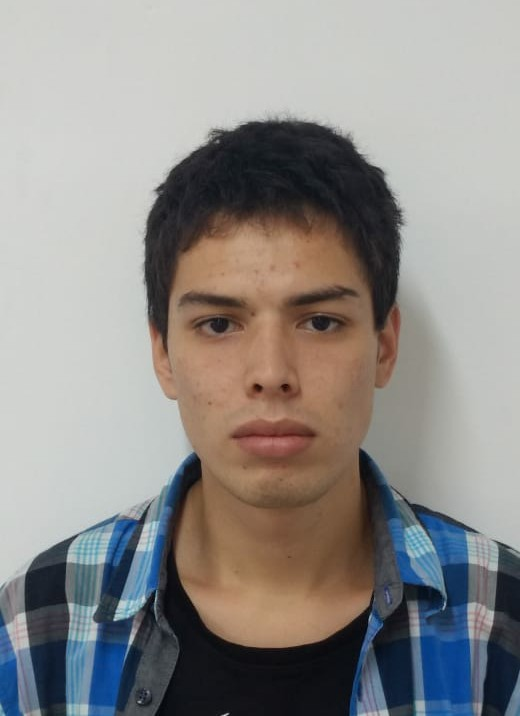
\includegraphics[scale=0.2]{img/Photo.png}
  \section{Datos}
    CC:1040752177
    Nacimiento:14/02/1996
    ~
  \section{Dirección}
    guayabal,
    CR 53 CL9ASUR-23
    ~
  \section{Tel \& Skype}
    +57 3045589531  
    edwinalexis1996
    ~
  \section{Mail}
    \href{mailto:edwinalexis1996@gmail.com}{\textbf{edwinalexis1996@}\\gmail.com}
    ~
  \section{Web \& Git}
    \href{https://github.com/Alexised}{github.com/Alexised}
    ~
  \section{Programacion}
    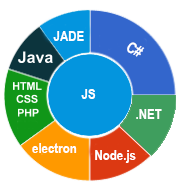
\includegraphics[scale=0.62]{img/programming.png}
    ~
  \section{Preferencias en Lenguajes}
    \textbf{js}
\includegraphics[scale=0.40]{img/5stars.png}
    \textbf{NODE.JS}
\includegraphics[scale=0.40]{img/5stars.png}
    \textbf{HTML}
\includegraphics[scale=0.40]{img/4stars.png}
    \textbf{CSS}
\includegraphics[scale=0.40]{img/4stars.png}
    ~
   ~
  \section{Idiomas}
    \textbf{English}
\includegraphics[scale=0.40]{img/3stars.png}
    ~
\end{aside}

\section{Perfil}
\begin{entrylist}
  \entry
    {}
    {Profesional \vspace{\baselineskip}}
    {  }
    {\emph{Me identifico como una persona responsable, trabajadora, dedicada, dinámica, respetuosa, honesta, que se compromete con los objetivos, dispuesta a cumplir metas tanto personales como grupales. Aprendo rápido, cumplo con lo que se me indica y realizo mis actividades de manera eficiente. De igual forma me caracterizo por ser una persona confiable. Siempre busco aprender conceptos nuevos y adquirir nuevas habilidades.\vspace{\baselineskip}
}}
  \entry
    {  }
    {Desarrollador \vspace{\baselineskip}}
    { }
    {\emph{He adquirido habilidades y competencias en diversos lenguajes de programación en el cual constantemente estoy en un proceso de actualizacion de conceptos nuevos y contenido, debido a mi particular gusto por las nuevas tecnologias y lenguajes de programacion,
    \\conocimientos en 
    Frameworks: Boopstrap, Materialize
    DB: SQL, MySQL, Mongo
}}
  
\end{entrylist}
\section{Educación}
\begin{entrylist}
  \entry
    {Semestre 5}
    {Tecnologia en Sistemas De Información}
    {Instituto Tecnológico Metropolitano, Medellin}
    {Objeto de formación.\\
    El objeto de formación del tecnólogo en desarrollo de software son las áreas de conocimiento en desarrollo de software y la administración de sistemas de información, logrando competencias para intervenir en adecuado manejo de la información haciendo un adecuado uso de la tecnología a nivel organizacional. Es un profesional ético de sólida formación integral en el campo científico, técnico y tecnológico, autónomo, capacitado para la toma de decisiones y capaz de trabajar en equipos multidisciplinarios.\\}
\end{entrylist}

\section{Certificaciones}
\begin{entrylist}
  \entry
    {2018}
    {Diploma-programación-básica}
    {Platzi}
    {\emph{curso de programacion en js }}
     \entry
    {2018}
    {Desarrollo de Apps Web}
    {Universidad Politécnica de Madrid}
    {\emph{Desarrollo en HTML5, CSS y Javascript de Apps Web, Android, IOS}}
\end{entrylist}
\section{Conferencias y Seminarios}
\begin{entrylist}
  \entry
    {2018}
    {PlatziTalks Medellín 2018}
    {Platzi}
    {\emph{ }}
     \entry
    {2017}
    {Medellin js}
    {Ruta N}
    {\emph{}}
\end{entrylist}
\newpage
\section{Experiencia Laboral}

\begin{entrylist}
  \entry
    {04/18 - 2019 }
    {Ingeniero Parametrizador}
    {Enterdev, Medellin, Colombia}
    {Diseño y desarrollo de algoritmos, Diseño y Desarrollo de procesos automatizados (RPA) con el uso de javascript, .net, wpf, C\#. \\}

\end{entrylist}

\begin{aside}
~
~
~
    ~
\end{aside}


\section{Referencias Personales}
Stiven Diaz Agudelo\\
\textbf{Desarrollador de aplicaciones }\\
\emph{Accenture}\\
\emph{Teléfono:3003510524}
\\

Jorge  Gonzalez Prada                                              \\
\textbf{Supervisor  }\\
\emph{Emtelco}\\
\emph{Teléfono:3183459032}\\

Sebastian Ruiz Lopera         \\
\textbf{Ingeniero Fisico Eafit}\\
\emph{Eafit}\\
\emph{Teléfono:3146776415 }
\\
\section{Referencias Laborales}
Juan Carlos sepulveda\\
\textbf{Ingeniero Parametrizadore}\\
\emph{Enterdev}\\
\emph{Teléfono:3134731278}
\\

Daniel Quintero Álvarez                                              \\
\textbf{Ingeniero Parametrizador }\\
\emph{Enterdev}\\
\emph{Teléfono:3166950531}
\\



\begin{flushleft}
\emph{}
\end{flushleft}
\begin{flushright}
\emph{}
\end{flushright}



\end{document}
